Let $F_n$ denote the free group of rank  $n$, generated by  $A \coloneq \Set{a_1,\ldots,a_n} $.
Let $U_n$ denote the free product of $n$ copies of  $\Z /2\Z$.
This should be thought of as the \emph{universal Coxeter group of rank  $n$}, since all rank  $n$ Coxeter groups are naturally a quotient of  $U_n$.
Let $S \coloneq \Set{s_1,\ldots,s_n} $ be the natural generating set for $U$, such that each  $s_i$ generates the  $i^\text{th}$ free factor.
For the whole of this document,  $n$ will be constant and arbitrary, so we will drop  $n$ from the above two notations, preferring just  $F$ and $U$.

A reflection in $F$ is a conjugate of any $f_i$ in $F$.
Denote the set of all reflections in $F$ by $R$.
Similarly, a reflection in $U$ is a conjugate of  any  $s_i$ in $U$.
Denote the set of all reflections in $U$ by  $T$.
So, a reflection in $U$ is some word $wu_i w^{-1}$, where $w=u_1\ldots u_k$ is a word in $S$.
We may assume $ws_iw^{-1}$ is a reduced word.
Thus, since every generator in $S$ is of order 2, we may assume that $w$ is a positive word where each factor has exponent  $+1$,  i.e.~each $u_i \in S$, and each $u_i$ is not equal to  $u_{i+1}$.

Since we will be using this notation a lot, let $s_i: w$ denote  $ws_iw^{-1}$.
Let $\phi \colon F \to U$ be the surjective homomorphism defined by $a_i \mapsto u_i$.
A lift of a reflection $s_i : w$ in $U$ is a choice of a positive or negative power for each $u_i$ in $w$, i.e.~a choice of a length $2k +1$ element in $\phi^{-1}(s_i : w) \cap R$.

Let $\C_n$ denote $\C \setminus \Set{z_1,\ldots,z_n}$.
Our free group $F$ is $\pi_1(\C_n, z_0)$ for any  $z_0 \notin \Set{z_1,\ldots,z_n} $.
We make the choice of $\Set{z_1,\ldots,z_n}$ to be $n$ evenly spaced points on the imaginary axis and within the unit circle, and $z_0 = -1$.
We draw a line $\lambda_i$ from each  $z_i$ to $z_0$.
For reasons that will become clear, we draw these lines in a roundabout way.

\begin{figure}[h]
	\centering
	\definecolor{ca2a2a2}{RGB}{162,162,162}
\definecolor{c848484}{RGB}{132,132,132}
\definecolor{c819d43}{RGB}{129,157,67}
\definecolor{c979797}{RGB}{151,151,151}

  \node[line width=0.01cm,anchor=south west] (text3024) at (7.0445, 24.7689){};



  \path[draw=ca2a2a2,line width=0.0183cm,dash pattern=on 0.0549cm off 0.0183cm] (4.7728, 22.7456) circle (1.3225cm);



  \node[text=black,line width=0.005cm,anchor=south west] (text27967) at (4.3552, 23.5882){$z_n$};



  \path[draw=c848484,line width=0.0039cm,dash pattern=on 0.0039cm off 0.0312cm] (4.7728, 24.2008) -- (4.7728, 21.239);



  \path[draw=c848484,line width=0.0039cm,dash pattern=on 0.0039cm off 0.0312cm] (6.2474, 22.7452) -- (3.2535, 22.7452);



  \node[text=black,line width=0.005cm,anchor=south west] (text57948) at (4.3552, 22.3656){$z_2$};



  \node[text=black,line width=0.005cm,anchor=south west] (text57988) at (3.0874, 22.7717){$z_0$};



  \node[text=black,line width=0.005cm,anchor=south west] (text57948-6) at (4.3552, 21.9507){$z_1$};



  \node[line width=0.0183cm,dash pattern=on 0.0549cm off 0.0183cm,anchor=south west] (text65615) at (4.6007, 22.6203){};



  \node[text=black,line width=0.005cm,rotate=-90.0,anchor=south west] (text66017) at (4.7001, 23.2334){$\ldots$};



  \node[text=black,line width=0.005cm,rotate=-98.3177,anchor=south west] (text72262) at (5.807, 23.1374){$\ldots$};



  \node[text=black,line width=0.005cm,anchor=south west] (text75234) at (5.7001, 23.3678){$\scriptstyle\lambda_n$};



  \node[text=black,line width=0.005cm,anchor=south west] (text75238) at (5.5759, 22.3416){$\scriptstyle\lambda_2$};



  \node[text=black,line width=0.005cm,anchor=south west] (text75242) at (5.4124, 21.9459){$\scriptstyle\lambda_1$};



  \path[draw=c819d43,line width=0.0139cm] (4.7709, 23.5501).. controls (5.1843, 23.4411) and (5.5979, 23.333) .. (6.0117, 23.2259).. controls (6.2449, 23.1655) and (6.4874, 23.1006) .. (6.6682, 22.9414).. controls (6.8034, 22.8224) and (6.894, 22.6562) .. (6.9324, 22.4802).. controls (6.9707, 22.3041) and (6.9582, 22.1187) .. (6.9079, 21.9457).. controls (6.8072, 21.5996) and (6.5626, 21.3122) .. (6.2878, 21.0789).. controls (6.0005, 20.8351) and (5.6708, 20.6371) .. (5.3109, 20.5254).. controls (4.951, 20.4138) and (4.56, 20.3911) .. (4.1959, 20.488).. controls (3.8317, 20.5849) and (3.497, 20.8056) .. (3.2868, 21.1184).. controls (3.0766, 21.4311) and (2.9992, 21.8362) .. (3.1052, 22.1978).. controls (3.1666, 22.4076) and (3.2876, 22.5996) .. (3.4504, 22.7456);



  \path[draw=black,fill=c979797,line width=0.0487cm] (4.7709, 23.5501) circle (0.0458cm);



  \path[draw=c819d43,line width=0.0139cm] (4.7709, 22.3547).. controls (5.1841, 22.3508) and (5.5972, 22.3274) .. (6.0082, 22.2846).. controls (6.0682, 22.2784) and (6.1285, 22.2716) .. (6.1864, 22.255).. controls (6.2444, 22.2383) and (6.3004, 22.2111) .. (6.3433, 22.1686).. controls (6.3835, 22.1287) and (6.4107, 22.0764) .. (6.4238, 22.0212).. controls (6.4369, 21.966) and (6.4363, 21.908) .. (6.4258, 21.8523).. controls (6.4048, 21.7408) and (6.3454, 21.6403) .. (6.2798, 21.5478).. controls (6.0943, 21.2862) and (5.8486, 21.0659) .. (5.563, 20.9201).. controls (5.2774, 20.7743) and (4.9518, 20.7044) .. (4.6323, 20.7314).. controls (4.3127, 20.7584) and (4.0005, 20.8839) .. (3.7584, 21.0942).. controls (3.5163, 21.3045) and (3.3471, 21.5998) .. (3.2991, 21.9169).. controls (3.2562, 22.1996) and (3.3103, 22.4962) .. (3.4504, 22.7456);



  \path[draw=c819d43,line width=0.0139cm] (4.7709, 21.9165).. controls (5.1023, 21.9469) and (5.4387, 21.9232) .. (5.7626, 21.8466).. controls (5.8161, 21.834) and (5.87, 21.8196) .. (5.918, 21.7926).. controls (5.9659, 21.7656) and (6.008, 21.7243) .. (6.0254, 21.6721).. controls (6.0352, 21.6426) and (6.0368, 21.6105) .. (6.0318, 21.5798).. controls (6.0267, 21.549) and (6.0151, 21.5195) .. (5.9995, 21.4926).. controls (5.9682, 21.4387) and (5.9215, 21.3955) .. (5.8732, 21.3562).. controls (5.5099, 21.06) and (5.0086, 20.9368) .. (4.5518, 21.0419).. controls (4.095, 21.147) and (3.6947, 21.4815) .. (3.5203, 21.9165).. controls (3.4156, 22.1777) and (3.3909, 22.4703) .. (3.4504, 22.7453);



  \path[draw=black,fill=c979797,line width=0.0487cm] (4.7709, 21.9169) circle (0.0458cm);



  \path[draw=black,fill=c979797,line width=0.0487cm] (4.7709, 22.3547) circle (0.0458cm);



  \path[draw=black,fill=c979797,line width=0.0487cm] (3.4501, 22.7409) circle (0.0458cm);




	\caption{Arrangement of $n+1$ points on the sphere, illustrating  $\tilde{\C}_n$.}
\end{figure}

We should think of these lines meeting  $z_0$ somehow, as in the
We can put these points on the sphere.

\begin{figure}[h]
	\centering
	
\definecolor{c66b814}{RGB}{102,184,20}
\definecolor{c979797}{RGB}{151,151,151}


\def \globalscale {1.000000}
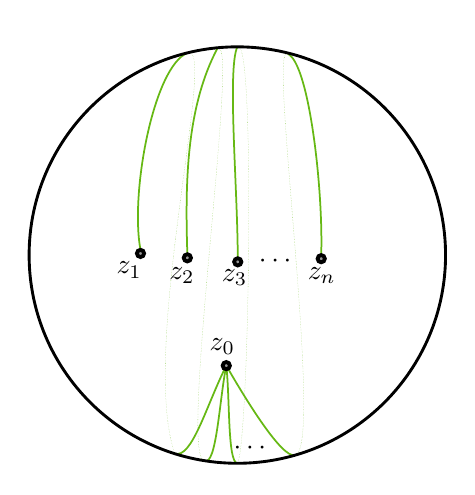
\begin{tikzpicture}[y=1cm, x=1cm, yscale=\globalscale,xscale=\globalscale, every node/.append style={scale=\globalscale}, inner sep=0pt, outer sep=0pt]
  \path[draw=c66b814,line width=0.0222cm] (5.4807, 24.8004).. controls (5.3448, 25.5198) and (5.6476, 27.1272) .. (6.0776, 27.3017);



  \path[draw=c66b814,line width=0.0222cm] (6.0756, 24.7445).. controls (6.0488, 25.6046) and (6.0524, 26.5901) .. (6.4553, 27.3542);



  \path[draw=c66b814,line width=0.0222cm] (7.7757, 24.7339).. controls (7.8018, 25.583) and (7.6202, 27.1582) .. (7.3542, 27.288);



  \path[draw=c66b814,line width=0.0222cm] (6.7159, 24.6936).. controls (6.7141, 25.5886) and (6.5814, 27.0922) .. (6.7105, 27.3785);



  \node[line width=0.01cm,anchor=south west] (text3024) at (7.0445, 24.7689){};



  \path[draw=c66b814,line width=0.0222cm] (6.5702, 23.3296).. controls (6.317, 22.8264) and (6.1359, 22.1459) .. (5.9161, 22.2118);



  \path[draw=c66b814,line width=0.0222cm] (6.5702, 23.3296).. controls (6.484, 22.9122) and (6.4468, 22.0498) .. (6.2945, 22.1226);



  \path[draw=c66b814,line width=0.0222cm] (6.5702, 23.3296).. controls (6.617, 22.9163) and (6.5852, 22.1039) .. (6.7105, 22.0896);



  \path[draw=c66b814,line width=0.0222cm] (6.5702, 23.3296).. controls (6.8311, 22.8757) and (7.2765, 22.1551) .. (7.4404, 22.1924);



  \path[draw=c66b814,line width=0.004cm,dash pattern=on 0.004cm off 0.016cm] (6.0776, 27.3017).. controls (6.4711, 27.4723) and (5.4597, 23.5454) .. (5.9161, 22.2118);



  \path[draw=c66b814,line width=0.004cm,dash pattern=on 0.004cm off 0.016cm] (7.3456, 27.2794).. controls (7.0986, 27.4722) and (7.822, 22.242) .. (7.4404, 22.1924);



  \path[draw=c66b814,line width=0.004cm,dash pattern=on 0.004cm off 0.016cm] (6.7105, 27.3785).. controls (6.9475, 27.5998) and (6.8581, 22.272) .. (6.7105, 22.0896);



  \path[draw=c66b814,line width=0.004cm,dash pattern=on 0.004cm off 0.016cm] (6.4553, 27.3542).. controls (6.7562, 27.6202) and (5.956, 22.1207) .. (6.2945, 22.1226) -- (6.2945, 22.1226);



  \path[draw=black,fill=c979797,line width=0.0487cm] (6.5702, 23.3296) circle (0.0458cm);



  \path[draw=black,line width=0.0365cm] (6.7105, 24.7341) circle (2.6444cm);



  \node[text=black,line width=0.01cm,anchor=south west] (text25704) at (6.665, 22.2053){$\cdots$};



  \node[text=black,line width=0.01cm,anchor=south west] (text28085) at (6.3593, 23.4682){$z_0$};



  \path[draw=black,fill=c979797,line width=0.0487cm] (5.4807, 24.7547) circle (0.0458cm);



  \path[draw=black,fill=c979797,line width=0.0487cm] (6.0756, 24.6988) circle (0.0458cm);



  \path[draw=black,fill=c979797,line width=0.0487cm] (6.7159, 24.6479) circle (0.0458cm);



  \path[draw=black,fill=c979797,line width=0.0487cm] (7.7757, 24.6881) circle (0.0458cm);



  \node[text=black,line width=0.01cm,anchor=south west] (text3028) at (6.9854, 24.5772){$\cdots$};



  \node[text=black,line width=0.01cm,anchor=south west] (text27967) at (5.1768, 24.442){$z_1$};



  \node[text=black,line width=0.01cm,anchor=south west] (text28077) at (5.8461, 24.3723){$z_2$};



  \node[text=black,line width=0.01cm,anchor=south west] (text28081) at (6.5154, 24.3477){$z_3$};



  \node[text=black,line width=0.01cm,anchor=south west] (text28089) at (7.6049, 24.3723){$z_n$};




\end{tikzpicture}
 % ← Path to the exported file
	\caption{Arrangement of $n+1$ points on the sphere, illustrating  $\tilde{\C}_n$.}
\end{figure}
